\documentclass[a4paper]{article}
\usepackage[pdftex]{graphicx}
\usepackage[utf8]{inputenc}
\usepackage{enumerate}
\usepackage{amssymb}
\usepackage{colortbl}
\usepackage{icomma}
\usepackage{siunitx}
\sisetup{locale=DE}
\usepackage{geometry}
\geometry{a4paper, top=15mm, left=15mm, right=15mm, bottom=15mm, 
	headsep=10mm, footskip=12mm}
\usepackage{href-ul}
\hypersetup{ 
	colorlinks=true, 
	linkcolor=blue,
	urlcolor=blue}
\usepackage{tikz}
\usetikzlibrary{positioning}
\usepackage{circuitikz}

\begin{document}
	
	{\bf Branched Circuits}
	
	\begin{enumerate}[1.]
		
		\begin{minipage}{0.75\textwidth}
			\item You have the following light bulbs to choose from: \\ Complete the missing technical data!
			\vspace{0.5 cm}
			
			\renewcommand{\arraystretch}{2}
			\begin{tabular}{|c|c|c|c|c|}
				\hline
				& Voltage U & Power P & Operating Current I & Resistance R \\
				\hline
				$L_1$ & 6 V & 0.6 W & & \\
				\hline
				$L_2$ & 6 V & 1.8 W & & \\
				\hline
				$L_3$ & 3.5 V & 0.7 W & & \\
				\hline
			\end{tabular}
		\end{minipage}
		\begin{minipage}{0.2 \textwidth}
			
			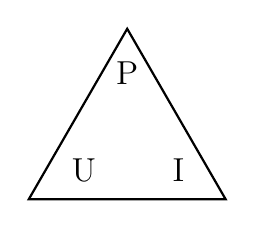
\begin{tikzpicture}[scale=1]
				% Triangle with side length 2.5 cm
				\coordinate (U) at (0,0);
				\coordinate (I) at (2.5,0); 
				\coordinate (P) at (1.25, {2.5*sqrt(3)/2}); 
				
				% draw lines 
				\draw[thick] (U) -- (I) -- (P) -- cycle; 
				
				% label inside 
				\node[above=0.1cm of U, xshift=0.7cm] {\large U}; 
				\node[above=0.1cm of I, xshift=-0.6cm] {\large I}; 
				\node[below=0.3cm of P] {\large P}; 
			\end{tikzpicture} 
			\vspace{0.5 cm} 
			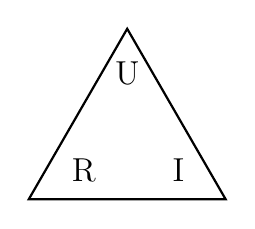
\begin{tikzpicture}[scale=1] 
				% triangle with side length 2.5 cm 
				\coordinate (R) at (0,0); 
				\coordinate (I) at (2.5,0);
				\coordinate (U) at (1.25, {2.5*sqrt(3)/2});
				
				% Draw lines
				\draw[thick] (R) -- (I) -- (U) -- cycle;
				
				% Label within
				\node[above=0.1cm of R, xshift=0.7cm] {\large R};
				\node[above=0.1cm of I, xshift=-0.6cm] {\large I};
				\node[below=0.3cm of U] {\large U};
			\end{tikzpicture}
		\end{minipage}
		
		You have eight AAA 1.5 V batteries as the power source, which you can connect in series.
		\item Enter possible combinations of lamps and power sources into the circuits so that they illuminate optimally!
		What is the total current then? \\
		How many batteries are you using as each voltage source?\\
		What is the total resistance of the circuit? \\
		
		\begin{minipage}{0.5\textwidth}
			{\bf Circuit A}
			
			\begin{circuitikz}[american]
				% battery (negative bottom, positive top), then series lamp L1,
				% then node with two lamps (L2 and L3) in parallel, back to negative.
				\draw
				(0,0) node[ground]{} % Negative (ground)
				to[battery1,l=$U$] (0,3) % Battery
				to[lamp] (3,3) node(N){} % Series lamp L1 and node N
				-- (5,3) % Connection to the upper branch point
				% First parallel branch (left)
				(3.5,3) to[lamp] (3.5,0) -- (0,0)
				% Second parallel branch (right)
				(5,3) to[lamp] (5,0) -- (0,0)
				;
			\end{circuitikz}
			
			\renewcommand{\arraystretch}{2}
			\begin{tabular}{|p{1.6 cm}|p{1.6 cm}|p{1.6 cm}|p{1.6 cm}|}
				\hline
				$U_{ges}$ & $I_{ges}$ & $R_{ges}$ & $P_{ges}$ \\
				\hline
				& & & \\
				\hline
			\end{tabular}
		\end{minipage}
		\begin{minipage}{0.5\textwidth}
			{\bf Circuit B}
			
			\begin{circuitikz}[american]
				% battery (negative bottom, positive top), then series lamp L1,
				% then node with two lamps (L2 and L3) in parallel, back to negative.
				\draw
				(0,0) node[ground]{} % Negative (ground)
				to[battery1,l=$U$] (0,3) % Battery
				to[lamp] (3,3) node(N){} % Series lamp L1 and node N
				-- (6.5,3) % Connection to the upper branch point
				% First parallel branch (left)
				(3.5,3) to[lamp] (3.5,0) -- (0,0)
				% Second parallel branch (right)
				(5,3) to[lamp] (5,0) -- (0,0)
				% Third parallel branch (right)
				(6.5,3) to[lamp] (6.5,0) -- (0,0)
				;
			\end{circuitikz}
			
			\renewcommand{\arraystretch}{2}
			\begin{tabular}{|p{1.6 cm}|p{1.6 cm}|p{1.6 cm}|p{1.6 cm}|}
				\hline
				$U_{ges}$ & $I_{ges}$ & $R_{ges}$ & $P_{ges}$ \\
				\hline
				& & & \\
				\hline
			\end{tabular}
		\end{minipage}
		\vspace{0.5 cm}
		
		\item Explain why, with the given lamps, only two identical lamps in a series circuit make sense.
		\item Now, {\bf two different lamps are connected in series}.
		For each combination of power source and lamps in the table, assess why it doesn't make sense and describe your observations.
		
		\renewcommand{\arraystretch}{2}
		\begin{tabular}{|c|c|p{12 cm}|}
			\hline
			Voltage U & Combination & Observation \\
			\hline
			3 V & $L_3$ + $L_1$ & \\
			\hline
			3 V & $L_3$ + $L_2$ & \\
			\hline
			4.5 V & $L_3$ + $L_2$ & \\
			\hline
			6 V & $L_3$ + $L_1$ & \\
			\hline
			6 V & $L_1$ + $L_2$ & \\
			\hline
		\end{tabular}
		
		\newpage
		
		\item Two lamps are now connected in parallel.
		For each combination of power source and lamps in the table, assess whether it makes sense and describe your observation.
		
		\renewcommand{\arraystretch}{2}
		\begin{tabular}{|c|c|p{12 cm}|}
			\hline
			Voltage U & Combination & Observation \\
			\hline
			3 V & $L_3$ + $L_3$ & \\
			\hline
			3 V & $L_3$ + $L_1$ & \\
			\hline
			3 V & $L_3$ + $L_2$ & \\
			\hline
			6 V & $L_1$ + $L_2$ & \\
			\hline
		\end{tabular}
		
		\end{enumerate}
		
		\fbox{
		\begin{minipage}{0.5\textwidth}
			% For the solution, please \href{https://www.okuyakl.de/phys/m/ll.pdf}{click here} or scan the QR code scan.\\ 
			Additional worksheets are available at 
			
			\href{https://www.okuyakl.de}{www.okuyakl.de} 
		\end{minipage} 
		\hfill 
		\begin{minipage}{0.4\textwidth} 
			\includegraphics[width=1.5 cm]{../../viecher/zwe03} 
			% \includegraphics[width=3 cm]{qr221} 
			\includegraphics[width=2 cm]{../../viecher/afanticon1} 
			
			\end{minipage}}
			
	\end{document}